\section{Monitoreo y Control del Proyecto}

El presente numeral describe los mecanismos que el equipo de desarrollo del Kit Pagos Colombia utilizará para conocer el estado de salud del proyecto en todo momento, detectar desviaciones respecto a lo planeado y ejecutar acciones correctivas oportunas. Los procesos aquí definidos son transversales a todas las fases del ciclo de vida DSR y operan en paralelo con la ejecución técnica del proyecto.

\subsection{Administración de Requerimientos}

El propósito de este proceso es garantizar que cualquier cambio en los requerimientos del producto sea detectado, evaluado, trazado y controlado de forma sistemática, de modo que el equipo y el director del proyecto conozcan en todo momento el estado de los requerimientos y las implicaciones de cualquier modificación sobre el alcance, el cronograma y los entregables.

\subsubsection{Artefactos del proceso}

Los artefactos que se producen y mantienen como resultado de la administración de requerimientos son los siguientes.

El primero es el Documento de Especificación de Requerimientos de Software (SRS), que constituye la línea base de requerimientos del proyecto. Este documento recoge los requerimientos funcionales organizados por componente, las historias de usuario con sus criterios de aceptación y los requerimientos no funcionales bajo la clasificación FURPS+. El SRS se considera un ítem de configuración y cualquier modificación sobre él debe seguir el proceso de control de cambios descrito en la sección 7.3.

El segundo es la Matriz de Trazabilidad de Requerimientos, que vincula cada requerimiento del SRS con el o los componentes del framework que lo implementan, con las pruebas que lo verifican y con el hito del ciclo de vida al que pertenece. Esta matriz permite detectar requerimientos huérfanos, componentes sin cobertura de prueba y el impacto de un cambio sobre el resto del sistema. La herramienta de soporte es Google Spreadsheets y su actualización es responsabilidad del integrante que asume el rol de ingeniero de requerimientos en cada fase.

El tercero es el Registro de Cambios de Requerimientos, un log mantenido en Notion que registra cada solicitud de cambio recibida, su estado (pendiente, aprobada, rechazada, implementada) y la referencia al pull request o al commit que materializó el cambio aprobado.

\subsubsection{Proceso de administración de requerimientos}

El proceso opera bajo las siguientes reglas. Cualquier integrante del equipo o el director puede proponer una modificación a los requerimientos. La propuesta se registra en Notion con una descripción del cambio, la justificación y el impacto estimado sobre el cronograma y los entregables. El equipo evalúa la propuesta en la reunión semanal y decide por consenso si se aprueba, se rechaza o se posterga. Si el director del proyecto ha solicitado el cambio, su aprobación es requisito necesario antes de proceder. Un cambio aprobado actualiza el SRS, la Matriz de Trazabilidad y el backlog de GitHub Projects en ese orden. Ningún cambio sobre la rama principal del repositorio se acepta sin que el SRS esté actualizado.

El diagrama BPMN del proceso de administración de requerimientos, que incluye los roles participantes, los puntos de decisión y los artefactos que se crean o refinan en cada paso, se presenta en la Figura~\ref{fig:bpmn-requerimientos}.

\begin{figure}[H]
  \centering
  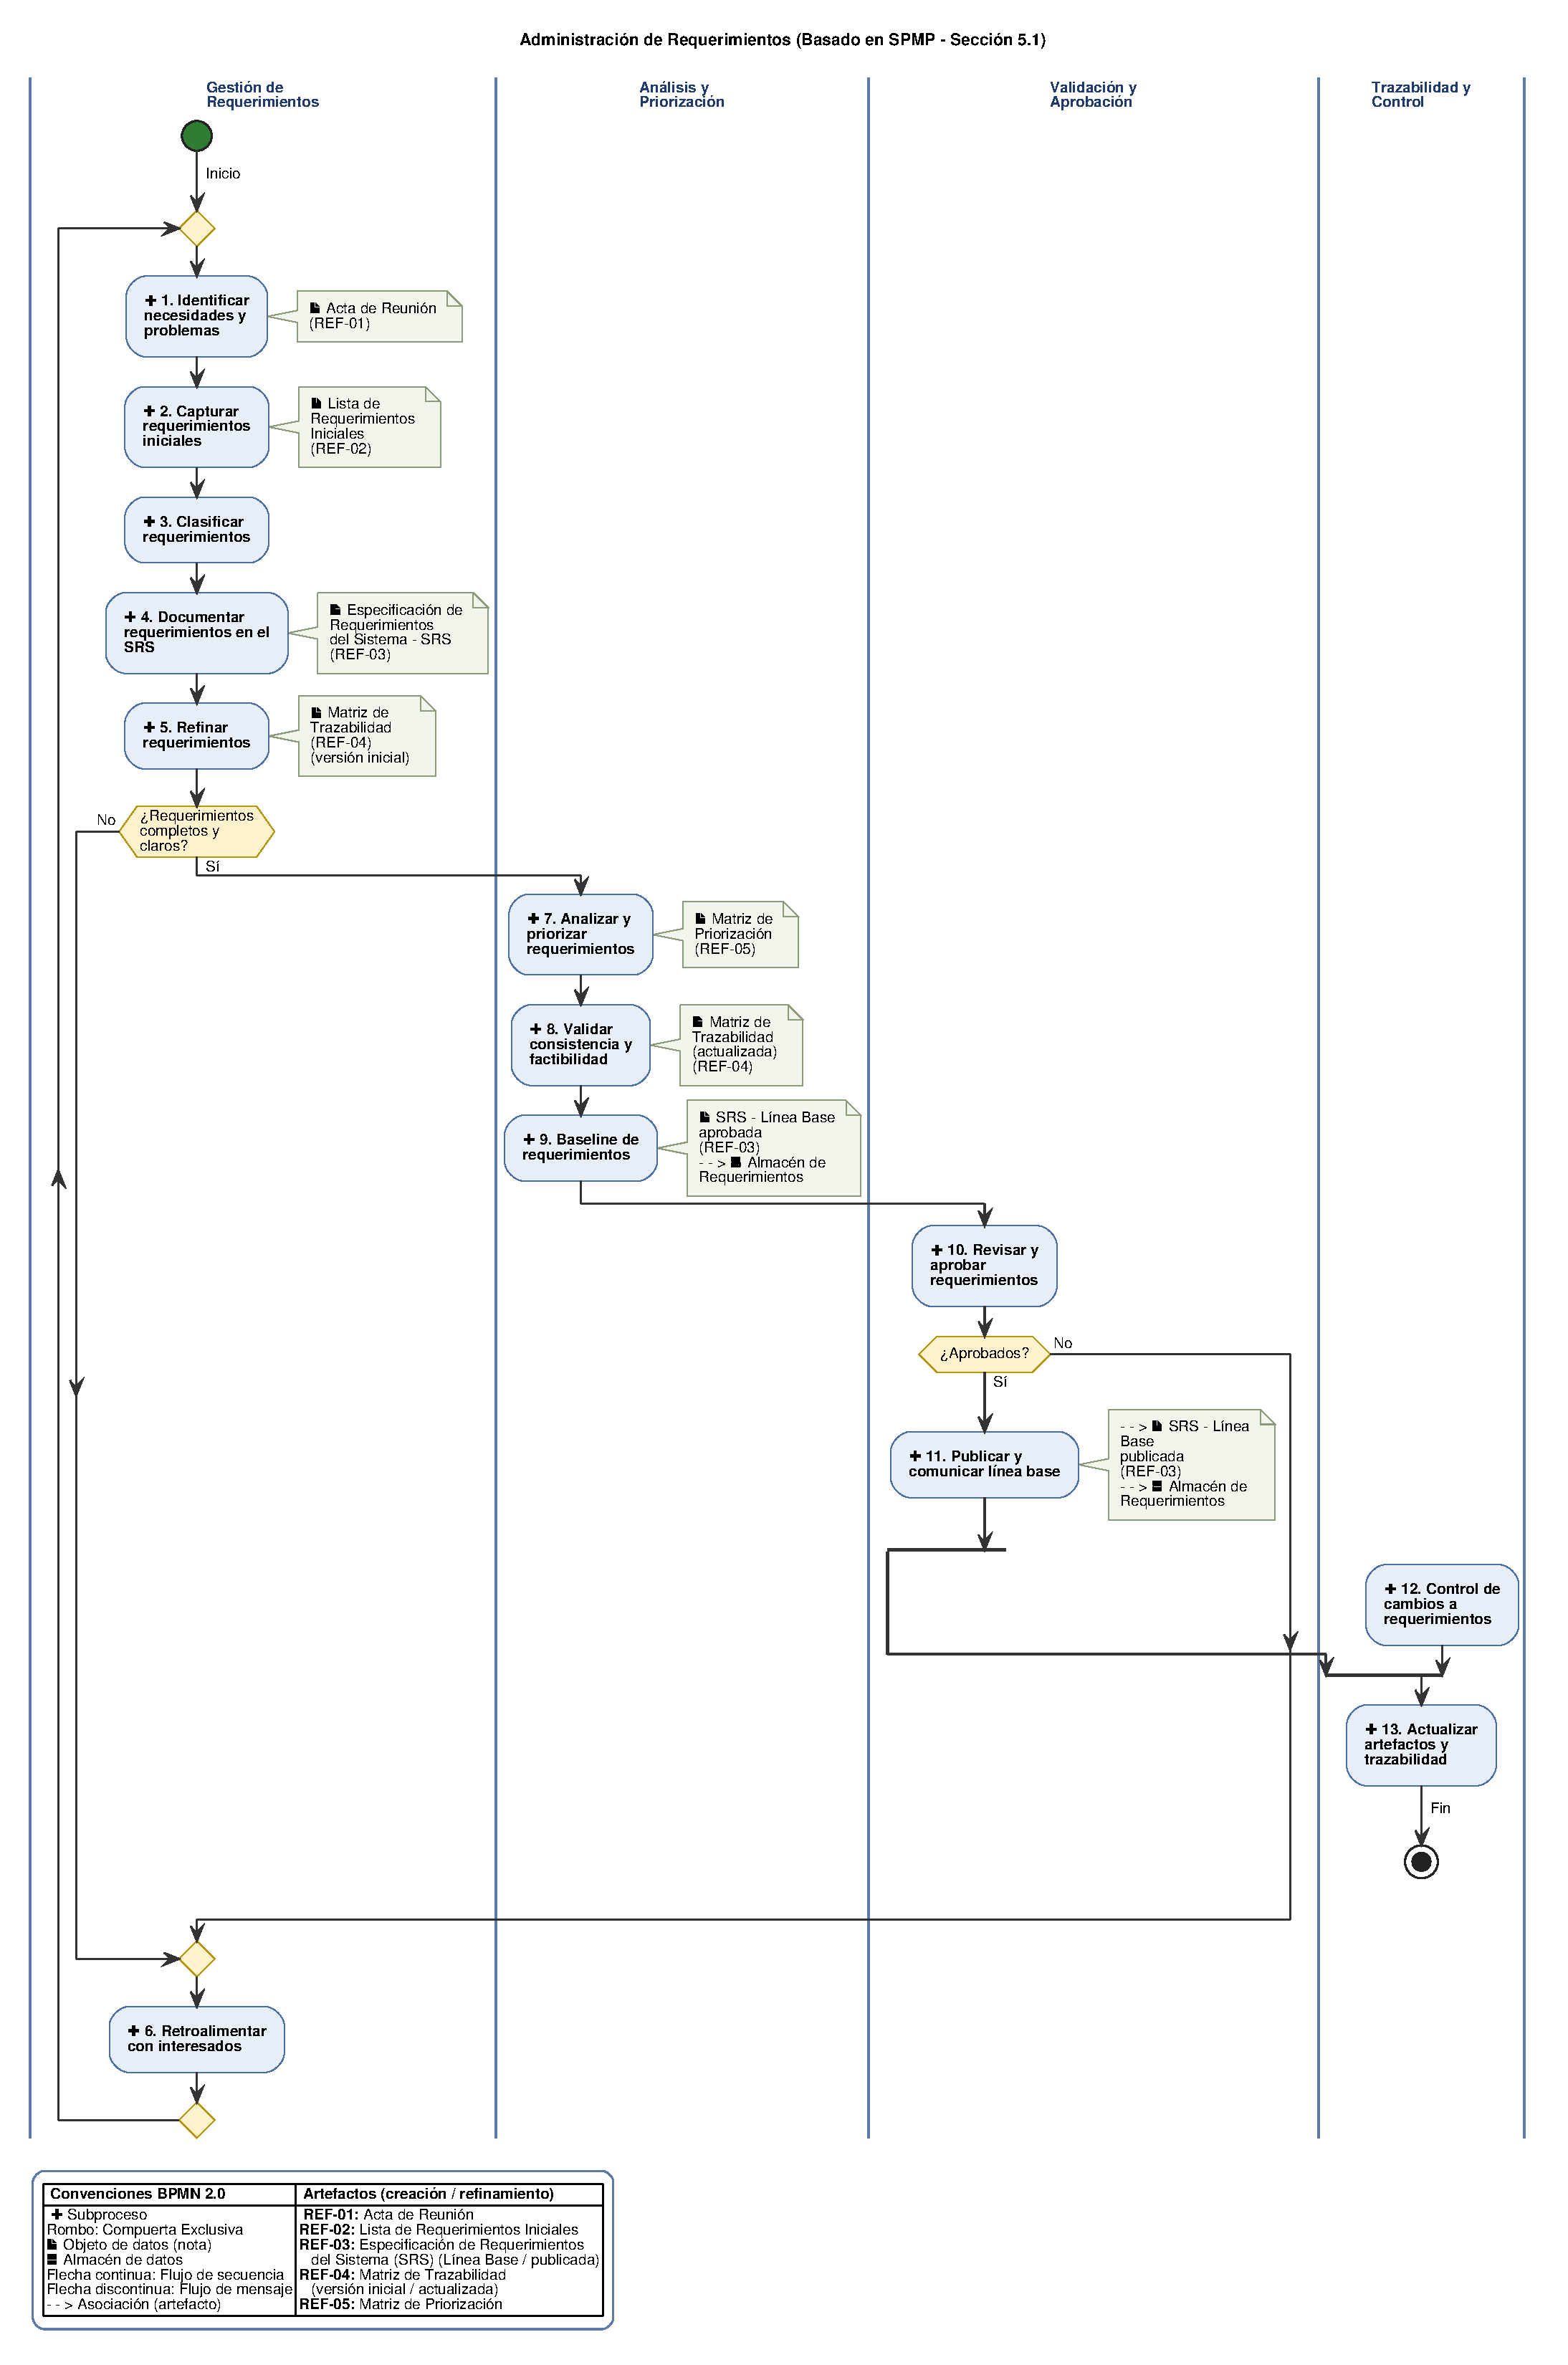
\includegraphics[width=\textwidth]{figuras/05-bpmn-requerimientos}
  \caption{Diagrama BPMN administración de requerimientos}
  \label{fig:bpmn-requerimientos}
\end{figure}

\subsection{Monitoreo y Control de Progreso}

El propósito de este proceso es proveer al equipo y al director del proyecto de información objetiva y periódica sobre el avance real del proyecto frente al plan establecido, y definir las acciones correctivas que se ejecutarán cuando el progreso no sea el esperado.

\subsubsection{Unidades de medición del progreso}

El progreso del proyecto se mide a través de las siguientes métricas.

La tasa de completitud del backlog se expresa como el porcentaje de ítems del backlog de GitHub Projects marcados como completados respecto al total de ítems planificados para la fase en curso. Un ítem se considera completado cuando su pull request asociado ha sido aprobado y mergeado a la rama principal. Esta métrica se revisa semanalmente.

El estado de los hitos del ciclo de vida es una métrica binaria que indica si cada uno de los seis hitos definidos en la sección 3.1.3 ha sido alcanzado o no en la fecha comprometida. Los hitos son los puntos de referencia más gruesos del proyecto y su incumplimiento activa el protocolo de acción correctiva.

La cobertura de pruebas del núcleo del SDK se expresa como el porcentaje de líneas de código del núcleo cubiertas por pruebas unitarias automatizadas, reportado por Jest al finalizar cada ejecución de la suite de pruebas en el pipeline de integración continua de GitHub Actions. El umbral mínimo aceptable es del 80\%, conforme a lo establecido en el Plan de Aceptación (sección 3.3.1).

El tiempo de respuesta de la API de simulación se mide en milisegundos desde el envío de la solicitud hasta la recepción de la respuesta completa, utilizando Postman o k6 desde una red estándar. Esta métrica se verifica en cada iteración de la fase de desarrollo y debe mantenerse por debajo de los 500ms para los escenarios sin latencia intencionada.

El número de defectos abiertos por componente se registra en GitHub Issues y se clasifica por componente (núcleo, adaptador Wompi, adaptador PayU, adaptador Mercado Pago, adaptador Kushki, API de simulación) y por severidad (bloqueante, mayor, menor). Esta métrica se revisa semanalmente.

\subsubsection{Actividades de reporte de progreso}

El progreso se reporta mediante las siguientes actividades periódicas.

La revisión semanal de backlog se realiza cada lunes al inicio de la semana de trabajo. Los cuatro integrantes actualizan el estado de sus ítems en GitHub Projects, registran los impedimentos encontrados y estiman el trabajo pendiente para la semana. La duración máxima de esta actividad es de 30 minutos. El responsable de convocarla es el integrante que asume el rol de coordinador en cada fase.

El reporte de progreso al director se entrega quincenalmente por correo electrónico o mediante reunión en Microsoft Teams, según la disponibilidad del director. El reporte incluye el estado de los hitos, la tasa de completitud del backlog, el estado de la cobertura de pruebas y los defectos abiertos por componente. La elaboración del reporte es responsabilidad del coordinador de la fase en curso.

La demostración al final de cada iteración de desarrollo se realiza internamente entre los cuatro integrantes al cierre de cada iteración de la fase de desarrollo (núcleo, adaptadores, API de simulación). En esta instancia se verifica que los criterios de aceptación de los ítems completados se cumplan efectivamente, y el resultado se registra en Notion.

Para que un requerimiento se considere implementado exitosamente, deben cumplirse simultáneamente las siguientes condiciones: el pull request asociado ha sido aprobado por al menos un integrante distinto al autor, las pruebas automatizadas relevantes pasan en el pipeline de CI, el ítem en GitHub Projects está en estado completado y la Matriz de Trazabilidad ha sido actualizada.

\subsubsection{Acciones correctivas}

El progreso del proyecto se mide a través de seis métricas principales, coherentes con las definidas en la sección 7.4 del presente documento. A continuación se describe cada una con su unidad de medición, su umbral de aceptación y el responsable de su recolección.

La completitud de tareas se expresa como el porcentaje de tareas del backlog de GitHub Projects marcadas como completadas respecto al total de tareas planificadas para la semana en curso. Una tarea se considera completada únicamente cuando su pull request asociado ha sido aprobado por al menos un integrante distinto al autor y mergeado a la rama de desarrollo. El target semanal es igual o superior al 80\%. Esta métrica la recolecta el coordinador cada viernes a las 5:00 p.m., revisando el tablero de GitHub Projects y registrando el porcentaje resultante en Google Spreadsheets bajo la hoja proyecto/metricas-semanales.

La cobertura de pruebas unitarias del núcleo se expresa como el porcentaje de líneas de código del núcleo del SDK cubiertas por pruebas unitarias automatizadas. El umbral mínimo aceptable es del 80\%, conforme a lo establecido en el Plan de Aceptación de la sección 3.3.1. Esta métrica la recolecta el líder de arquitectura y núcleo antes de cada merge a la rama de desarrollo, ejecutando jest --coverage en el pipeline de integración continua de GitHub Actions. El resultado se reporta automáticamente en el comentario del pull request correspondiente.

Las métricas de complejidad CK cuantifican las propiedades estructurales del código del framework mediante tres indicadores del conjunto de Chidamber y Kemerer: WMC (Weighted Methods per Class), con umbral máximo de 15; CBO (Coupling Between Object Classes), con umbral máximo de 5; y RFC (Response For a Class), con umbral máximo de 20. Estas métricas se calculan al cierre de cada iteración de desarrollo ejecutando un script de ts-morph que analiza el directorio src/ y genera un reporte JSON con los valores por clase. Los resultados se registran en Google Spreadsheets bajo la hoja proyecto/metricas-ck. La recolección es responsabilidad del líder de evaluación y documentación. La definición completa de estas métricas y su papel en la evaluación del artefacto se describe en la sección 7.4.

El cumplimiento de hitos es una métrica binaria que indica si cada uno de los seis hitos del ciclo de vida (H1 a H6) fue alcanzado dentro del rango de fecha permitido, definido como la fecha comprometida más o menos tres días. El coordinador verifica esta métrica en la reunión de sincronización de los jueves, contrastando el estado de los entregables asociados a cada hito frente a las fechas del cronograma de la sección 4.

Los defectos por artefacto en revisión contabilizan el número de comentarios clasificados como defecto, es decir, errores funcionales o estructurales y no meras sugerencias, encontrados durante la revisión de pull requests para código o durante la revisión por pares para documentos. El target es un máximo de dos defectos por artefacto antes de su aprobación. El líder de arquitectura y núcleo recolecta esta métrica para los artefactos de código y el líder de evaluación y documentación la recolecta para los artefactos documentales, clasificando cada defecto por tipo: lógico, de estilo o de cobertura.

El tiempo de resolución de impedimentos se expresa en días hábiles transcurridos entre el momento en que un impedimento se registra en Notion o GitHub Issues y el momento en que se marca como resuelto. El target para impedimentos críticos es de máximo dos días hábiles. Esta métrica la recolecta el coordinador semanalmente calculando la diferencia entre las fechas de reporte y resolución de cada impedimento registrado.

El progreso se reporta mediante las siguientes actividades:

La revisión semanal de backlog se realiza cada lunes a las 10:00 a.m. en la reunión de planificación del equipo. Los cuatro integrantes actualizan el estado de sus ítems en GitHub Projects, registran los impedimentos encontrados durante la semana anterior y estiman el trabajo pendiente para la semana que inicia. La duración máxima de esta actividad es de una hora. El coordinador es el responsable de convocarla, de calcular la tasa de completitud de la semana cerrada y de presentar un resumen de las métricas de progreso al equipo.

La sincronización de mitad de semana se realiza cada jueves a las 3:00 p.m. con duración máxima de 45 minutos. El coordinador presenta un resumen de las métricas de la semana en curso, se identifican impedimentos activos y se toman decisiones técnicas urgentes. Si en esta instancia se detecta una desviación significativa en alguna métrica, se convoca una sesión de análisis de causa raíz antes de la reunión del lunes siguiente. El acta queda registrada en Notion con las decisiones y compromisos acordados.

El reporte de progreso al director se entrega quincenalmente los viernes a las 4:00 p.m. mediante reunión en Microsoft Teams o por correo electrónico, según la disponibilidad del director. El reporte incluye el estado de los hitos del ciclo de vida, la tasa de completitud semanal acumulada de la quincena, la cobertura de pruebas del núcleo, los defectos abiertos por componente, los impedimentos activos y su tiempo de resolución, y los valores más recientes de las métricas CK cuando corresponda a la fase en curso. La elaboración del reporte es responsabilidad del coordinador y el director lo utiliza para validar que el progreso es adecuado y para autorizar cambios de alcance si es necesario.

La demostración al cierre de cada iteración de desarrollo se realiza internamente entre los cuatro integrantes al finalizar cada iteración de la fase de desarrollo (núcleo, adaptadores, API de simulación). En esta instancia se verifica que los criterios de aceptación de los ítems completados se cumplen efectivamente y se registra el resultado en Notion. Un requerimiento se considera implementado exitosamente cuando se cumplen simultáneamente las siguientes condiciones: el pull request asociado fue aprobado por al menos un integrante distinto al autor, las pruebas automatizadas relevantes pasan en el pipeline de CI con cobertura igual o superior al 80\%, el ítem en GitHub Projects está en estado completado, los valores de WMC, CBO y RFC de las clases modificadas están dentro de los umbrales definidos, y la Matriz de Trazabilidad ha sido actualizada para reflejar el requerimiento como implementado.

El reporte consolidado de cierre de fase se elabora al alcanzar cada uno de los hitos H1 a H6. El líder de evaluación y documentación prepara un reporte que incluye gráficas de tendencia de las métricas CK a lo largo de la fase, la evolución de la cobertura de pruebas, el cumplimiento de hitos, el número de defectos encontrados y resueltos, y el tiempo promedio de resolución de impedimentos. Este reporte forma parte del documento de trabajo de grado para análisis retrospectivo y se entrega al director junto con el entregable formal de la fase.

Las acciones correctivas se activan bajo las siguientes condiciones.

Cuando la tasa de completitud al cierre de una semana es inferior al 60\% de las tareas planificadas, el coordinador convoca dentro de las 24 horas siguientes una reunión extraordinaria de no más de una hora con todos los integrantes. En esta reunión se identifican las causas del retraso mediante un análisis de causa raíz, y se decide por consenso alguna de las siguientes acciones: redistribuir el trabajo entre integrantes con mayor disponibilidad, reducir el alcance del ítem afectado postergando funcionalidad no crítica a la siguiente iteración, o aumentar el tiempo de dedicación semanal de los integrantes involucrados. La decisión queda registrada en Notion con fecha, responsables y fecha de revisión de su efectividad. Si el retraso se origina en un impedimento técnico que ningún integrante puede resolver en menos de dos días hábiles, se escala al director del proyecto en la reunión quincenal o de forma inmediata si el impedimento bloquea el hito en curso.

Cuando un valor de WMC, CBO o RFC supera su umbral en alguna clase del framework durante la revisión del pull request, el líder de arquitectura y núcleo registra el hallazgo como defecto en el pull request y el código no se aprueba hasta que el autor resuelva la violación. Si la violación persiste en dos iteraciones consecutivas sobre la misma clase, se convoca una sesión técnica de refactorización con los integrantes involucrados en ese componente.

Cuando un hito no se alcanza en la fecha comprometida, el equipo elabora dentro de los dos días hábiles siguientes un plan de recuperación que especifica qué actividades se reordenarán, qué recursos adicionales se asignarán y en cuántas semanas se proyecta recuperar el retraso. Este plan se presenta al director en la reunión quincenal inmediatamente siguiente al incumplimiento del hito. En ningún caso se acuerdan reducciones de alcance que afecten los entregables comprometidos sin la aprobación explícita del director.

Cuando la cobertura de pruebas del núcleo cae por debajo del 80\% en cualquier ejecución del pipeline de CI, el pull request asociado se rechaza automáticamente y el autor es responsable de agregar las pruebas faltantes antes de solicitar una nueva revisión. Esta condición no es negociable y no requiere reunión de equipo para activarse.

\subsection{Cierre del Proyecto}

El propósito de esta sección es describir las acciones necesarias para cerrar formalmente cada fase del proyecto antes de cada entrega, así como las acciones de cierre final al término del semestre.

\subsubsection{Cierre de fase}

Al finalizar cada fase del ciclo de vida DSR, el equipo ejecuta las siguientes actividades previas a la entrega. Se realiza un post-mortem de la fase, de no más de una hora, en el que se identifican las actividades que funcionaron bien, las que presentaron dificultades y las mejoras que se incorporarán en la fase siguiente. Los resultados quedan registrados en Notion. Se verifica que todos los artefactos comprometidos para esa fase estén completos, actualizados y almacenados en los repositorios correspondientes (GitHub para el código y los documentos técnicos, Google Drive para los entregables académicos). Se elabora el reporte gerencial de la fase, que resume el trabajo realizado, el estado de los hitos, las métricas de progreso y las lecciones aprendidas, y se entrega al director junto con el entregable formal de la fase.

\subsubsection{Cierre final del proyecto}

Al término del semestre, el equipo ejecuta adicionalmente las siguientes acciones de cierre final: publicación del repositorio público del framework con documentación suficiente para que un desarrollador externo pueda integrar el kit sin haber participado en su desarrollo, entrega del documento de trabajo de grado en su versión final al director y a la facultad según los procedimientos académicos vigentes, y archivo de todos los artefactos del proyecto en los repositorios correspondientes con acceso habilitado para el director y los evaluadores académicos.
